\documentclass[11pt]{article}
\usepackage[margin=1in]{geometry}
\usepackage{graphicx}
\usepackage{float}
\usepackage{hyperref}
\usepackage{caption}
\title{Stock Market Analysis Report}
\author{Your Name}
\date{\today}

\begin{document}
\maketitle
\tableofcontents
\newpage

\section{Introduction}
This report summarizes the results of fetching, analyzing, and visualizing stock price data 
for several major tickers using R and the \texttt{quantmod} suite.  

\section{Methodology}
\begin{itemize}
  \item Daily adjusted closing prices downloaded from Yahoo Finance.
  \item Computation of 20-day and 50-day Simple Moving Averages.
  \item Calculation of daily log returns and 20-day rolling volatility.
  \item Generation of per-ticker charts and a comparative normalized performance plot.
\end{itemize}

\section{Key Figures}

\begin{figure}[H]
  \centering
  \includegraphics[width=\textwidth]{img/plot-01.png}
  \caption{AAPL Price with 20/50-day SMAs}
\end{figure}

\begin{figure}[H]
  \centering
  \includegraphics[width=\textwidth]{img/plot-03.png}
  \caption{AAPL Histogram of Daily Log Returns}
\end{figure}

\begin{figure}[H]
  \centering
  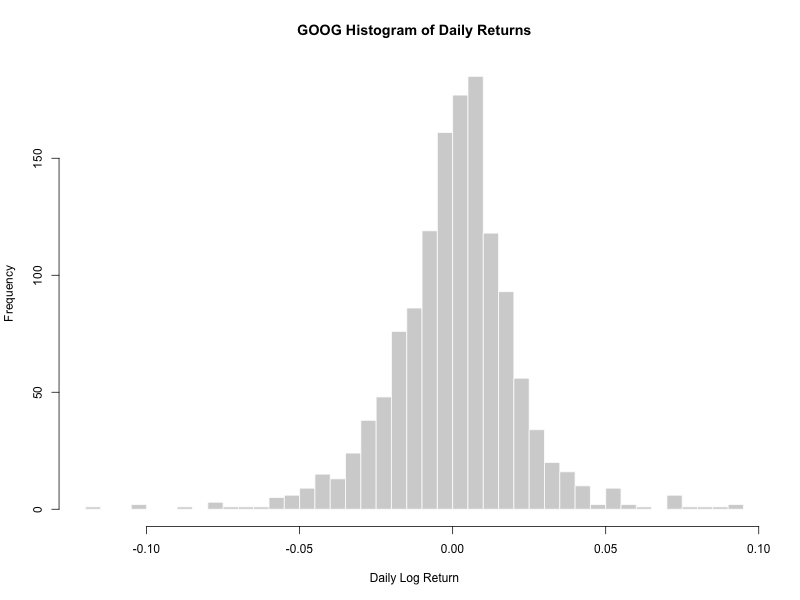
\includegraphics[width=\textwidth]{img/plot-15.png}
  \caption{GOOG 20-Day Rolling Volatility}
\end{figure}

\begin{figure}[H]
  \centering
  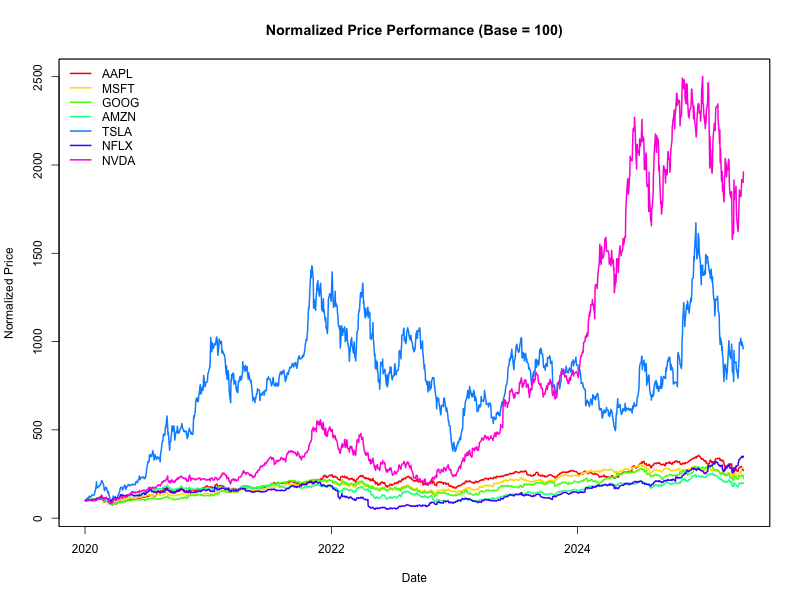
\includegraphics[width=\textwidth]{img/plot-43.png}
  \caption{Normalized Price Performance (Base = 100)}
\end{figure}

\section{Conclusions}
Summarize trends, volatility patterns, and cross‐ticker comparisons here.

\end{document}
